
\documentclass[a4paper]{scrreprt}
 
\usepackage[german]{babel}
\usepackage[utf8]{inputenc}
\usepackage[T1]{fontenc}
\usepackage{ae}
\usepackage[scaled]{helvet}
\renewcommand\familydefault{\sfdefault} 
\usepackage[onehalfspacing]{setspace}
\usepackage[scaled]{helvet}
\renewcommand*\familydefault{\sfdefault}
\usepackage[T1]{fontenc}
\usepackage{glossaries}
\usepackage{graphicx}
\usepackage[bookmarks,bookmarksnumbered]{hyperref}
\usepackage{float}
\usepackage[font={footnotesize}]{caption}
\usepackage{titlesec}
\titleformat{\paragraph}
{\normalfont\normalsize\bfseries}{\theparagraph}{1em}{}
\titlespacing*{\paragraph}
{0pt}{3.25ex plus 1ex minus .2ex}{1.5ex plus .2ex}
\setlength{\parindent}{0pt}%
\setcounter{tocdepth}{1} 
\setcounter{secnumdepth}{2} 
\makenoidxglossaries
\newglossaryentry{Server}
{	name=Server,
	description={Ein Server (englisch server, wörtlich Diener oder Bediensteter, im weiteren Sinn auch Dienst) ist ein Computerprogramm oder ein Computer, der Computerfunktionalitäten wie Dienstprogramme, Daten oder andere Ressourcen bereitstellt, damit andere Computer oder Programme („Clients“) darauf zugreifen können}
}
\newglossaryentry{App}
{ 	name=App,
	plural=Apps,
	description={Als Mobile App (auf Deutsch meist in der Kurzform die App, eine Abkürzung für den Fachbegriff Applikation) wird eine Anwendungssoftware für Mobilgeräte beziehungsweise mobile Betriebssysteme bezeichnet}
}
\newglossaryentry{Nutzer}
{	name=Nutzer,
	description={Ein Benutzer (auch Endbenutzer, Bediener oder kurz Nutzer genannt sowie englisch User) ist eine Person, die ein Hilfs- oder Arbeitsmittel zur Erzielung eines Nutzens verwendet, beispielsweise für eine Zeitersparnis oder Kostensenkung}
}
\newglossaryentry{Desktop Anwendung}
{	name=Desktop Anwendung,
	plural=Desktop Anwendungen,
	description={Als Desktop Anwendungen (auch Anwendungsprogramm, kurz Anwendung oder Applikation; englisch application software, kurz App) werden Computerprogramme bezeichnet, die genutzt werden, um eine nützliche oder gewünschte nicht systemtechnische Funktionalität zu bearbeiten oder zu unterstützen. Sie dienen der „Lösung von Benutzerproblemen“}
}
\newglossaryentry{Drag and Drop}
{	name=Drag and Drop,
	description={Drag and Drop, oft auch Drag’n’Drop, deutsch „Ziehen und Ablegen“, ist eine Methode zur Bedienung grafischer Benutzeroberflächen von Rechnern durch das Bewegen grafischer Elemente mittels eines Zeigegerätes. Ein Element wie z. B. ein Piktogramm kann damit gezogen und über einem möglichen Ziel losgelassen werden. Dieses kann zum Beispiel markierter Text oder das Symbol einer Datei sein }
}
\newglossaryentry{Medikament}
{	name=Medikament,
	description={Arzneimittel oder gleichbedeutend Medikamente (lateinisch medicamentum „Heilmittel“) sind Stoffe oder Stoffzusammensetzungen, die „zur Heilung oder zur Verhütung menschlicher oder tierischer Krankheiten bestimmt sind“ oder sich dazu eignen, physiologische Funktionen zu beeinflussen oder eine medizinische Diagnose zu ermöglichen}
}
\newglossaryentry{NFC}
{ 	name=NFC,
	description={Die Nahfeldkommunikation (Near Field Communication, abgekürzt NFC) ist ein auf der RFID-Technik basierender internationaler Übertragungsstandard zum kontaktlosen Austausch von Daten per elektromagnetischer Induktion mittels loser gekoppelter Spulen über kurze Strecken von wenigen Zentimetern}
}
\newglossaryentry{Versichertennummer}
{ 	name=Versichertennummer,
	description={Die Krankenversichertennummer dient der Identifikation des Versicherten bei einer Krankenversicherung. Die Krankenversichertennummer wird benötigt, damit Leistungserbringer, z. B. Ärzte oder Zahnärzte ihre Leistungen mittels der Krankenversicherungskarte, über die Kassenärztlichen Vereinigungen, mit der zuständigen Krankenkasse abrechnen können}
}
\newglossaryentry{Bluetooth}
{	name=Bluetooth,
	description={Bluetooth ist ein in den 1990er Jahren durch die Bluetooth Special Interest Group (SIG) entwickelter Industriestandard gemäß IEEE 802.15.1 für die Datenübertragung zwischen Geräten über kurze Distanz per Funktechnik (WPAN). Dabei sind verbindungslose sowie verbindungsbehaftete Übertragungen von Punkt zu Punkt und Ad-hoc- oder Piconetze möglich}
}
\newglossaryentry{Pop-Up}
{	name=Pop-Up,
	description={Ein Pop-up (von englisch to pop up, „plötzlich auftauchen“) ist ein Element einer grafischen Benutzeroberfläche. In der Regel werden Pop-ups eingesetzt, um zusätzliche Inhalte anzuzeigen oder eine bestimmte Interaktion abzufragen. Typischerweise „springen“ Pop-ups auf und überdecken dabei andere Teile der Benutzeroberfläche}
}
\newglossaryentry{Cloud}
{	name=Cloud,
	description={Die Cloud ist keine physische Größe, sondern ein riesiges Netzwerk aus Remoteservern, die über die ganzen Welt verteilt aber miteinander verbunden sind, damit sie als ein einziges großes Ökosystem funktionieren können}
}
\newglossaryentry{Tab}
{	name=Tab,
	description={Eine Registerkarte, auch Reiter oder Tab genannt, ist ein Steuerelement einer grafischen Benutzeroberfläche, das einem Registerblatt aus Aktenschränken nachempfunden wurde }
}
 
\newglossaryentry{Arztbrief}
{	name=Arztbrief,
	plural=Arztbriefe,
	description={Der Arztbrief, oft synonym als Epikrise, Entlassungsbrief, Patientenbrief oder Befundbericht bezeichnet, ist ein Transferdokument für die Kommunikation zwischen Ärzten. Der Arztbrief gibt einen zusammenfassenden Überblick über den Status des Patienten bei der Entlassung, einen Rückblick über den Krankheitsverlauf, die veranlasste Therapie, eine Interpretation des Geschehens zum Krankheitsverlauf im speziellen Fall}
}
\newglossaryentry{Anamnese}
{	name=Anamnese,
	description={Die Anamnese (von altgriechisch anámnēsis, deutsch ‚Erinnerung‘) ist die professionelle Erfragung von potenziell medizinisch relevanten Informationen durch Fachpersonal (z. B. einen Arzt)}
}
 
\begin{document}
\begin{titlepage}
\begin{figure}[h]
	\vspace{-4cm}
	\hspace{-2cm}
	
\includegraphics[ width=0.3\textwidth]{graphics/Kit_Logo}
	\label{fig:Aufg03_1}
\end{figure}
	\vspace{1.5cm}
	\centering
	
\includegraphics[width=0.5\textwidth]{graphics/myMD_Logo}\par\vspace{0.5cm}
	{\Huge myMD \par}
	\vspace{2cm}
	{\scshape\Large Implementierung\par}
	\vspace{1cm}
	Praxis der Softwareentwicklung WS2017/2018 \par
	\vspace{2cm}
	{\Large\itshape Philipp Pelcz, Philipp Karcher, Jan-Luca Vettel\par}
	\vfill
	supervised by \par
	Marc Aurel Kiefer
	\vfill
% Bottom of the page
	{\large \today \par}
\end{titlepage}
 
% Platzierung des Inhaltsverzeichnisses
\tableofcontents
\addtocontents{toc}{\protect\enlargethispage{10cm}}
\setlength{\parskip}{2.5mm}%
\chapter{Einleitung}
"myMD" ist eine mobile Anwendung, die es Patienten erlaubt ihre Arztbriefe digital über Bluetooth von ihren Ärzten zu erhalten, um dann in der Applikation die darin enthaltenen Informationen, wie die Diagnose oder verschrieben Medikationen, einsehen zu können.

Die App wurde dabei mit Xamarin.Forms in C\# und XAML für Android- und iOS-Geräte entwickelt.

Aufbauend auf dem vorangegangenen Pflichtenheft und dem Entwurfsdokument, wird in diesem Dokument der Fortschritt der Implementierung und die dabei vorgenommenen Änderungen an in Planung und Entwurf festgelegten Kriterien beschrieben.

Zunächst werden noch einmal die wichtigsten Ergebnisse aus Planungs- und Entwurfsphase aufgelistet und danach die daran in dieser Phase vorgenommenen Änderungen. Dazu zählen geänderte Entwürfe, Klassen und nicht umgesetzt Kriterien. 

Letztlich folgen noch abschließende Worte über den Verlauf der Phase und Pläne für die Zukunft.

\chapter{Vorangegangene Planung}
\section{Kriterien (Planungsphase)}
\textit{Hinweis: Der Übersicht wegen sind hier Pflicht- und Wunschkriterien zusammen aufgeführt. Sie sind weiterhin anhand der Kürzel voneinander unterscheidbar (PK = Pflichtkriterium WK = Wunschkriterium).}
\subsubsection{Patientenseitige Datenübertragung}
\begin{tabular}{lll}

[PK1010] & \multicolumn{2}{p{12cm}}  {\glspl{Arztbrief} können von der \gls{Desktop Anwendung} auf die myMD \gls{App} des Patienten übertragen werden.} \\
{[PK1020]} & \multicolumn{2}{p{12cm}}  {Die Übertragung erfolgt verschlüsselt über \gls{Bluetooth}.} \\
{[PK1030]} & \multicolumn{2}{p{12cm}}  {Eine laufende Datenübertragung kann manuell abgebrochen werden.} \\
{[WK1010]} & \multicolumn{2}{p{12cm}}  {Ein \gls{Arztbrief} kann von der myMD \gls{App} des Patienten auf die \gls{Desktop Anwendung} übertragen werden.} \\
{[WK1020]} & \multicolumn{2}{p{12cm}}  {Der Patient kann mehrere \glspl{Arztbrief} gleichzeitig senden.} \\
{[WK1030]} & \multicolumn{2}{p{12cm}}  {\gls{NFC} steht als weitere Übertragungsmöglichkeit zur Verfügung.} \\
{[WK1040]} & \multicolumn{2}{p{12cm}}  {Der Patient wird vor dem Senden von sensiblen Daten darauf hingewiesen, dass er sensible Daten versendet.} \\
{[WK1050]} & \multicolumn{2}{p{12cm}}  {Ein Profil auf einem Mobilgerät kann auf ein anderes übertragen werden.} \\

\end{tabular}

\subsubsection{Darstellung}
\begin{tabular}{lll}
[PK2010] & \multicolumn{2}{p{12cm}}  {\glspl{Arztbrief} werden chronologisch absteigend im \gls{Tab} \textit{Übersicht} dargestellt.} \\
{[PK2020]} & \multicolumn{2}{p{12cm}}  {Der \gls{Nutzer} kann überflüssige/unerwünschte \glspl{Arztbrief} löschen.} \\
{[PK2030]} & \multicolumn{2}{p{12cm}}  {Die Darstellung eines Arztbriefes umfasst die Diagnose, verordnete \gls{Medikament}e, das Datum und den Namen des behandelnden Arztes.} \\
{[WK2010]} & \multicolumn{2}{p{12cm}}  {Eingenommene \gls{Medikament}e werden in einem extra \gls{Tab} chronologisch absteigend sortiert dargestellt.} \\
{[WK2020]} & \multicolumn{2}{p{12cm}}  {Laborwerte des Patienten werden in einem extra \gls{Tab} chronologisch absteigend sortiert dargestellt.} \\
{[WK2030]} & \multicolumn{2}{p{12cm}}  {Ein \gls{Arztbrief} kann Bilddateien enthalten und die myMD \gls{App} kann diese originalgetreu darstellen und einem \gls{Arztbrief} zuordnen.} \\
{[WK2040]} & \multicolumn{2}{p{12cm}}  {Es gibt die Möglichkeit, \glspl{Arztbrief} nach eigenen Kriterien (Arzt, Krankheit o.ä.) zu gruppieren.} \\
{[WK2050]} & \multicolumn{2}{p{12cm}}  {Es gibt eine Suchfunktion, die alle \glspl{Arztbrief} nach Daten durchsucht.} \\
\end{tabular}

\subsubsection{Einstellungen}
\begin{tabular}{lll}
[PK3010] & \multicolumn{2}{p{12cm}}  {Der \gls{Nutzer} kann ein eigenes Profil anlegen, welches Daten wie den Namen, Versicherungsnummer, Blutgruppe und Allergien enthält.} \\
{[PK3020]} & \multicolumn{2}{p{12cm}}  {Die myMD \gls{App} wird in Deutsch angeboten.} \\
{[WK3010]} & \multicolumn{2}{p{12cm}}  {Auf einer myMD \gls{App} können mehrere \gls{Nutzer} verwaltet werden.} \\
{[WK3020]} & \multicolumn{2}{p{12cm}}  {Die myMD \gls{App} wird zusätzlich auch auf Englisch angeboten.} \\
{[WK3030]} & \multicolumn{2}{p{12cm}}  {Der \gls{Nutzer} kann einzelne \glspl{Arztbrief} oder ganze Gruppen als sensibel markieren.} \\
{[WK3040]} & \multicolumn{2}{p{12cm}}  {Die myMD \gls{App} kann den \gls{Nutzer} an regelmäßige Arzttermine (z.B. Zahnarzt, Augenarzt) erinnern.} \\

\end{tabular}

\subsubsection{\gls{Desktop Anwendung}}
\begin{tabular}{lll}
{[PK4010]} & \multicolumn{2}{p{12cm}}  {Die \gls{Desktop Anwendung} kann die Geräte in der Nähe anzeigen.} \\
{[PK4020]} & \multicolumn{2}{p{12cm}}  {Der Arzt kann unter den Geräten in der Nähe das Mobilgerät des Patienten als Empfänger auswählen.} \\
{[PK4030]} & \multicolumn{2}{p{12cm}}  {Digitale \glspl{Arztbrief} können entweder per \gls{Drag and Drop} oder über einen Explorer in die \gls{Desktop Anwendung} geladen werden.} \\
{[PK4040]} & \multicolumn{2}{p{12cm}}  {Die Daten werden auf Knopfdruck an das Mobilgerät des Patienten gesendet.} \\
{[WK4010]} & \multicolumn{2}{p{12cm}}  {Die \gls{Versichertennummer}, die in einem \gls{Arztbrief} auf dem Computer des Arztes eingetragen ist, wird vor dem Senden mit der in der myMD App des Patienten hinterlegten \gls{Versichertennummer} abgeglichen und nur bei Übereinstimmung wird der \gls{Arztbrief} gesendet.} \\
\end{tabular}

\subsubsection{Kompatibilität}
\begin{tabular}{lll}
[PK5010] & \multicolumn{2}{p{12cm}}  {Die \gls{Desktop Anwendung} wird von Microsoft Windows 10 unterstützt.} \\
{[PK5020]} & \multicolumn{2}{p{12cm}}  {Die myMD \gls{App} wird von Android 6.0 (und höher) unterstützt.} \\
{[PK5030]} & \multicolumn{2}{p{12cm}}  {Die myMD \gls{App} kann \glspl{Arztbrief} im .hl7 Dateiformat anzeigen.} \\
{[WK5010]} & \multicolumn{2}{p{12cm}}  {Die myMD \gls{App} wird von iOS 10 (und höher) unterstützt.} \\
{[WK5020]} & \multicolumn{2}{p{12cm}}  {Die \gls{Desktop Anwendung} wird zusätzlich von macOS 10.12 (und höher) unterstützt.} \\
{[WK5030]} & \multicolumn{2}{p{12cm}}  {Die myMD \gls{App} kann \gls{Arztbrief}e im .pdf Dateiformat anzeigen.} \\
{[WK5040]} & \multicolumn{2}{p{12cm}}  {Die myMD \gls{App} kann \gls{Arztbrief}e im .csv Dateiformat anzeigen.} \\

\end{tabular}

\section{Klassendiagramm (Entwurfsphase)}
\begin{figure}[H]
\hspace{-1.8cm}
\begin{minipage}[c]{\textwidth}
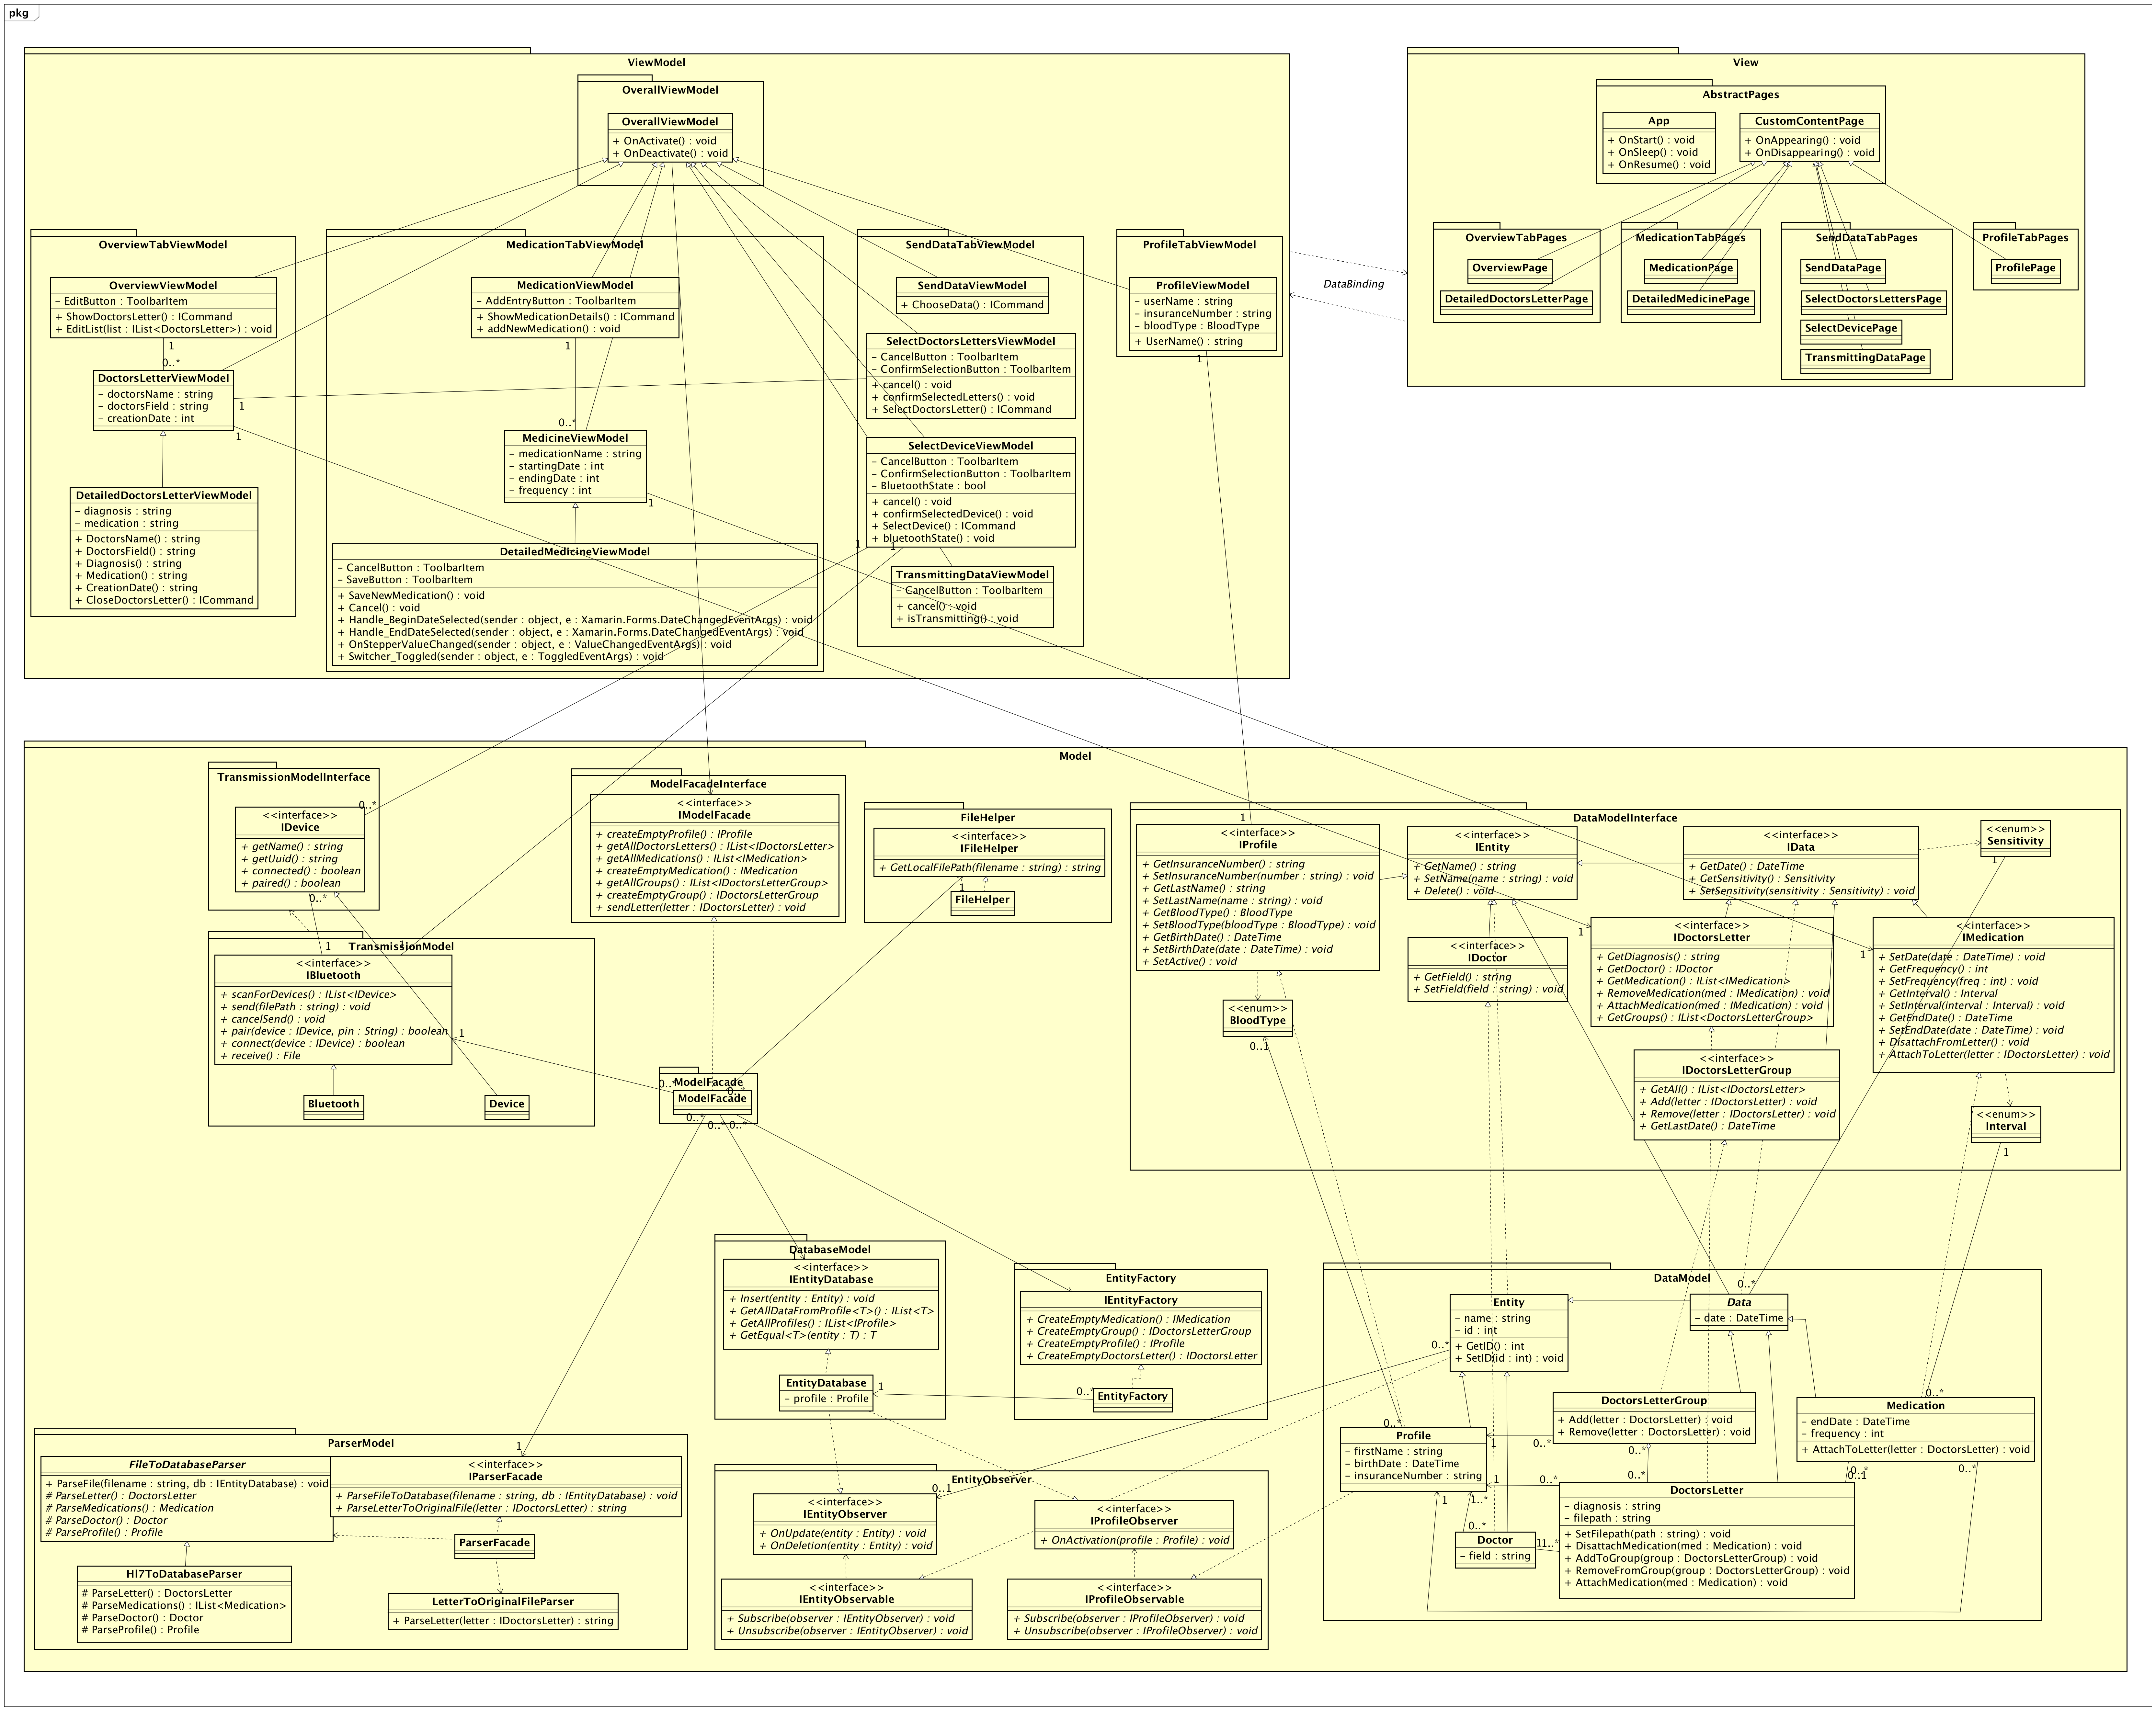
\includegraphics[width=1.6\textwidth, angle=90]{graphics/Klassendiagramme/myMD}
\caption{myMD Klassendiagramm der Entwurfsphase}
\end{minipage}
\end{figure}

\begin{figure}
\section{Gantt-Diagramm (Entwurfsphase)}
\begin{minipage}[c]{\textwidth}
\centering
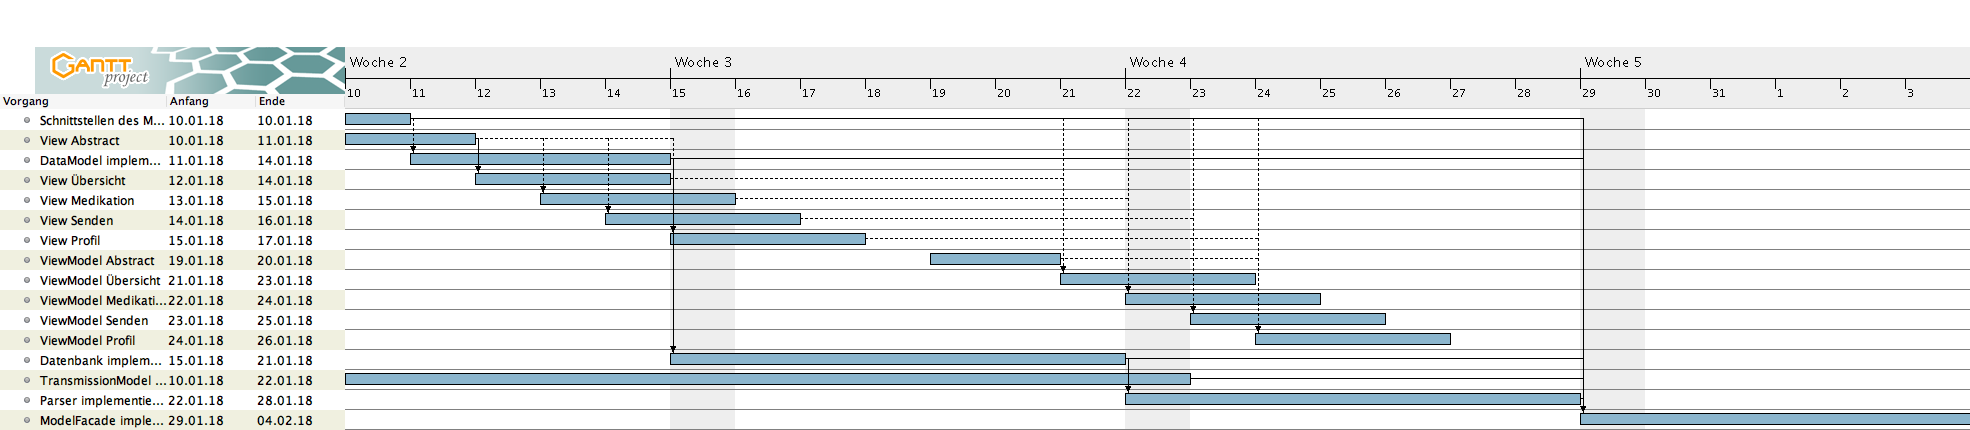
\includegraphics[width=0.95\textheight, angle=90]{Gantt/GanttChart}
\caption{Gantt Diagramm der Entwurfsphase}
\end{minipage}
\end{figure}

\chapter{Geänderte Daten}
\section{Geänderte Entwürfe}
\subsection{Model}
\subsubsection{Beobachter-Entwurfsmuster}
In der Entwurfsphase entschieden wir uns für das Beobachter-Entwurfsmuster, um die Datenbank über Änderungen an den Instanzen der Klassen aus dem \textbf{DataModel} Paket zu benachrichtigen.

Das \textbf{EntitiyObserver} Paket, das die dafür vorgesehenen Schnittstellen enthält, wurde mitsamt diesen komplett enfernt. Stattdessen muss das Aktualisieren einer Entität nun per explizitem Aufruf an die \textbf{ModelFacade} durchgeführt werden.

Die Gründe dafür sind zweigeteilt:

Erstens werden durch die Benutzung der \textit{SQLite-Net-Extensions} Library beim rekursiven Auflösen von Relationen Objekte aus der Datenbank geladen, ohne dass bei ihnen von uns die Datenbank als Beobachter angemeldet werden kann. Um das Laden von in Relation stehender Entitäten aus der Datenbank zu vereinfachen, ist es sinnvoll das Beobachterprinzip nicht weiter zu verwenden.

Zweitens ist es von der GUI-Seite auch intuitiver, Änderungen dann erst zu übernehmen, wenn dies explizit vom Benutzer so veranlasst wird. Damit bietet sich die \textit{Update} Methode in der \textbf{ModelFacade} als Alternative an.

\subsubsection{Datenbanktabellen}
Alle Klassen aus dem \textbf{DataModel} Paket stellen Vorlagen für eine Datenbanktabelle dar. Im ursprünglichen Entwurf waren nur die Getter und Setter für den Zugriff vom ViewModel aus vorgesehen (mit den Schnittstellen aus \textbf{DataModelInterface} als Parameter). Um Objekte vollständig in die Datenbank schreiben und wieder daraus laden zu können,  werden Getter und Setter für alle konkreten Attribute benötigt.

Um unnötiges Casten zu vermeiden, erhalten die Schnittstellen aus \textbf{DataModelInterface} noch eine Konvertierungsmethode zu der in \textbf{DataModel} definierten konkreten Implementierung (für die Klassen aus \textbf{DataModel} gibt diese Methode lediglich die Instanz der Klasse selbst zurück.)

\subsubsection{Plattformspezifisches Parsen}
\begin{figure}[H]
\centering
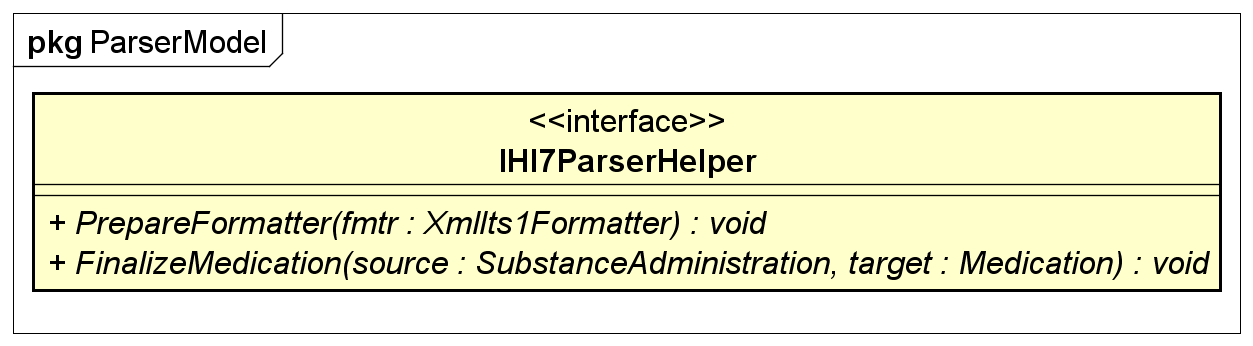
\includegraphics[width=0.75\textheight]{graphics/Klassendiagramme/Model/IHl7ParserHelper.png}
\caption{IHl7ParserHelper Schnittstelle}
\end{figure}
Bestimmte Klassen des \textit{Everest} Frameworks, das zum Parsen von .hl7 Dateien benutzt wird, implementieren die \textbf{ICloneable} Schnittstelle, die in einem \textit{Xamarin-Cross-Platform} Projekt nicht verfügbar ist. 

Manche dieser Klassen werden jedoch benötigt um die Dateien vollständig zu parsen, daher kann der \textbf{Hl7ToDatabaseParser} nicht mehr wie geplant komplett plattformunabhängig implementiert werden.

Operationen mit diesen Klassen werden nun über die \textbf{IHl7ParserHelper} Schnittstelle aufgerufen und im \textbf{Hl7ParserHelper} plattformspezifisch implementiert.

\subsubsection{Dateiformatunabhänigiges Parsen}
\begin{figure}[H]
\centering
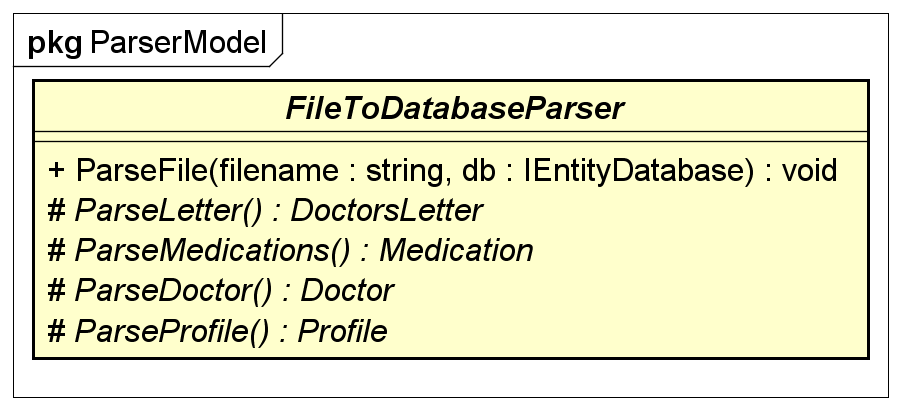
\includegraphics[width=0.75\textheight]{graphics/Klassendiagramme/Model/FileToDatabaseParser.png}
\caption{Klassen zum dateiformatunabhänigigen Parsen}
\end{figure}
Um in Zukunft die Implementierung der Unterstützung mehrere Dateiformate zu vereinfachen, wurden mehrere Änderungen am \textbf{FileToDabaseParser} vorgenommen:

Das Auswählen des richtigen Parsers erfolgt nun über die Enumeration \textbf{FileFormat} der unterstützen Dateiformate und eine Erweiterungsmethode in \textbf{FileFormatExtensions} die einem Dateiformat aus \textbf{FileFormat} den passenden \textbf{FileToDabaseParser} zuordnet.

Weiterhin wurden auch die dateiformatspezifischen Einschubmethoden des \textbf{FileToDabaseParser} modifiziert: 

Die zu parsende Datei wird nun über die neu hinzugefügte \textit{Init} Methode übergeben, die weiteren \textit{Parse} Methoden sind dafür nun parameterlos. Dies erlaubt es flexibler aus einer Datei lesen zu können. 

Beim vorherigen Ansatz musste für jeden Aufruf einer \textit{Parse} Methoden neu aus der Datei gelesen werden. Jetzt können stattdessen gemeinsame Vorbereitungen getroffen werden, wie z.B. beim \textbf{Hl7ToDatabaseParser}. Hier wird mit \textit{Init} die gesamte Datei mit \textit{Everest} in den frameworkeigenen Datentyp \textit{ClinicalDocument} geparst, der dann wiederum mit den restlichen \textit{Parse} Methoden in die Datentypen aus dem \textbf{DataModel} Paket geparst wird.

\subsection{ViewModel}
\subsubsection{Enum-Picker}
\begin{figure}[H]
\centering
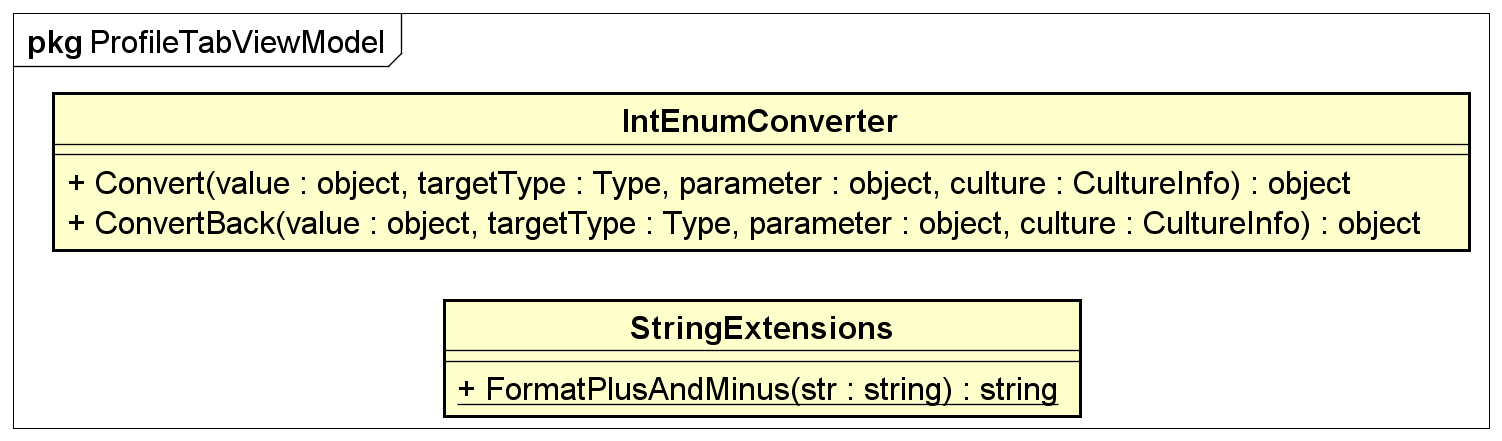
\includegraphics[width=0.75\textheight]{graphics/Klassendiagramme/ViewModel/Enum-Picker.png}
\caption{Enum Picker Klassen}
\end{figure}
Um Elemente aus einem Enum in einem Picker von \textit{Xamarin} darstellen zu können, wird ein Konvertierer (\textbf{IntEnumConverter}) benötigt, da die dafür von \textit{Xamarin} angebotene Funktionalität eine Liste von Elementen erwartet. Mit dem Konvertierer kann dann jedem Listeneintrag über \textit{DataBinding} ein Enum-Wert zugewiesen werden.

Um die Namen von Enumwerten zum Anzeigen formatieren zu können wurden für diesen Zweck auch noch die Klasse \textbf{StringExtensions} mit Erweiterungsmethoden für strings hinzugefügt.

\subsection{View}
\subsubsection{Benutzeroberflächenlogik}
In der Entwurfsphase orientierten wir uns daran, dass die Benutzeroberflächenlogik nach dem \textit{MVVM-Prinzip} in den jeweiligen \textit{ViewModeln} implementiert wird. Jedoch fiel uns auf, dass dies sehr umständlich ist. Deshalb haben wir die Benutzeroberflächenlogik im Code-Behind zu jeder entsprechenden Seite in der \textit{View} implementiert.
\subsubsection{ProfileEditPage}
Während dem Entwurf stellten wir uns vor, dass es auf einer \textbf{ProfilePage} einen Toggle zum Bearbeiten der Daten im Profil gibt, der die Labels, in denen die Daten stehen, durch Entrys ersetzt. Da sich diese Funktion, aber durch die Gestaltung der Seite in .xaml nur suboptimal implementieren lässt, haben wir uns dazu entschieden, die neue Seite \textbf{ProfileEditPage} einzuführen. Diese wird geöffnet, wenn man den \textit{Bearbeiten-Button
} der \textbf{ProfilePage} antippt. Die \textbf{ProfileEditPage} gleicht der \textbf{ProfilePage} im Design. Die Unterschiede begrenzen sich auf die zwei \textit{StatusBar-Elemente} \dq{}Abrechen\dq{}, \dq{}Fertig\dq{} und die Ersetzung der Labels (in der \textbf{ProfilPage}) durch Entrys.

\section{Geänderte Klassen}
\textit{Hinweis: Nur leicht (z.B. in der Namensgebung) geänderte Klassen oder solche, die bereits in den Geänderten Entwürfen erwähnt sind hier nicht aufgelistet. Weiterhin wurden die meisten Getter- und Setter-Methoden durch die in C\# üblichen Properties ersetzt. Da dies mehr eine optische als tatsächlich inhaltliche Änderung darstellt, wird auch dies hier übergangen.}

\subsection{ModelInterface}
\subsubsection{IModelFacade}
\begin{figure}[H]
\centering
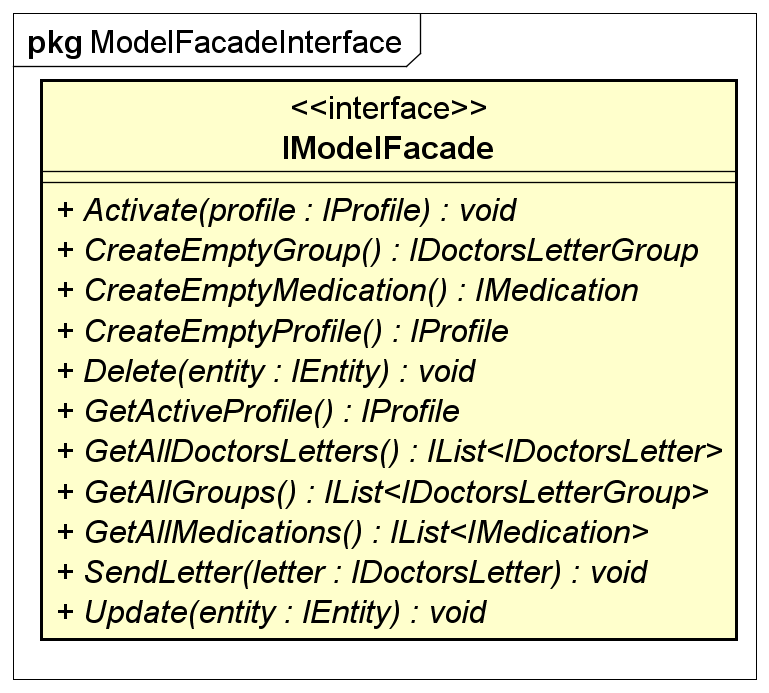
\includegraphics[width=0.75\textheight]{graphics/Klassendiagramme/Model/IModelFacade.png}
\caption{IModelFacade Schnittstelle}
\end{figure}
\textbf{Art der Änderung:} Neue Methoden

\textbf{Beschreibung:} Methode zum Abfragen des aktuell aktiven Profils hinzugefügt.

\textbf{Paket:} ModelInterface.ModelFacadeInterface

\subsubsection{IMedication}
\begin{figure}[H]
\centering
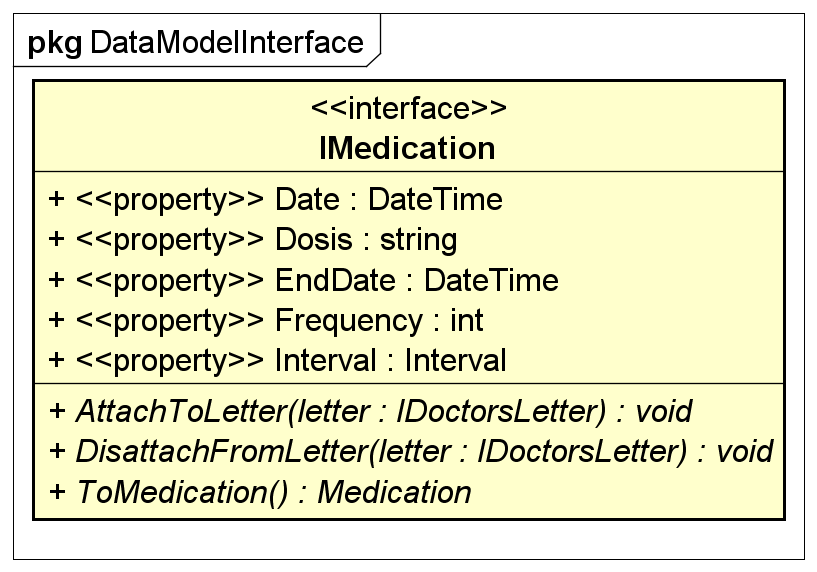
\includegraphics[width=0.75\textheight]{graphics/Klassendiagramme/Model/IMedication.png}
\caption{IMedication Schnittstelle}
\end{figure}
\textbf{Art der Änderung:} Neues Attribut

\textbf{Beschreibung:} Medikation haben jetzt auch eine Dosis (Getter und Setter als string)

\textbf{Paket:} ModelInterface.DataModelInterface

\subsection{Model}
\textit{Hinweis: Klassen aus dem \textbf{DataModel} Paket wurden Vergleichsmethoden wie Compare und Equals hinzugefügt, die hier nicht für jede Klasse einzeln aufgezählt werden.}

\subsubsection{IEntityDatabase}
\begin{figure}[H]
\centering
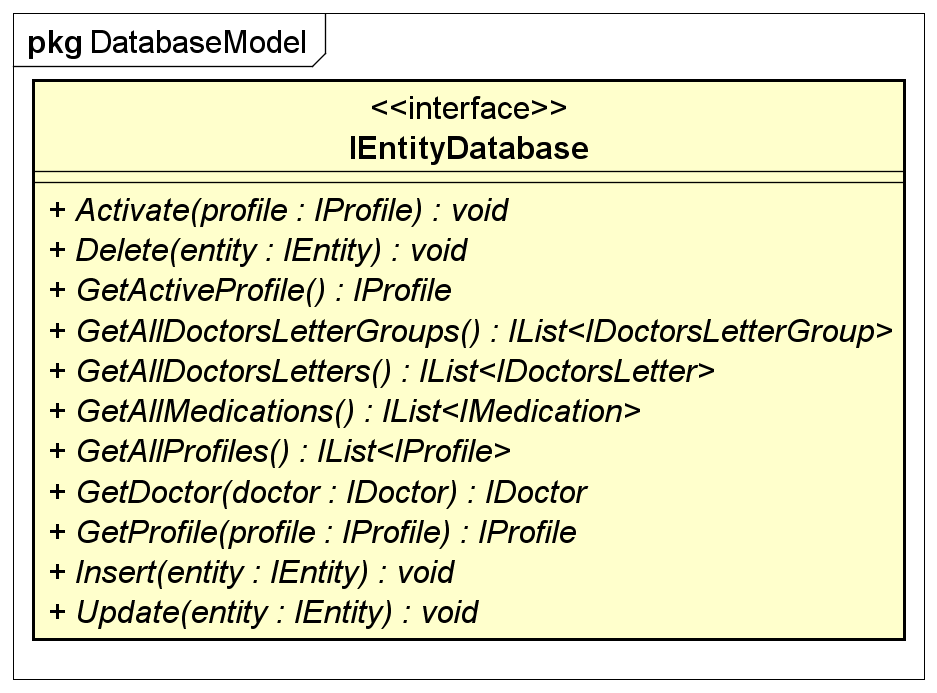
\includegraphics[width=0.75\textheight]{graphics/Klassendiagramme/Model/IEntityDatabase.png}
\caption{IEntityDatabase Schnittstelle}
\end{figure}
\textbf{Art der Änderung:} Neue/geänderte Methoden

\textbf{Beschreibung:} Die Methoden der Observer-Schnittstellen aus dem \textbf{EntityObserver} Paket befinden sich nun in dieser Schnittstelle. \\
Außerdem wurde die generischen Methoden durch typspezifische Methoden ersetzt, eine Methode zum Abfragen des aktuell aktiven Profils hinzugefügt und die Methodenparameter sind nun konsistent aus dem \textbf{DataModelInterface} Paket.

\textbf{Paket:} Model.EntityDatabase

\subsubsection{EntityFactory}
\begin{figure}[H]
\centering
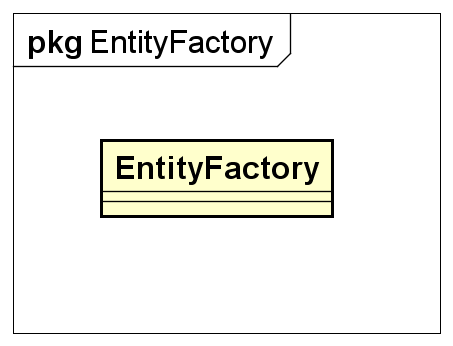
\includegraphics[width=0.75\textheight]{graphics/Klassendiagramme/Model/EntityFactory.png}
\caption{EntityFactory Klasse}
\end{figure}
\textbf{Art der Änderung:} Entferntes Attribut

\textbf{Beschreibung:} Im ursprünglichen Entwurf hatte \textbf{EntityFactory} noch eine \textbf{IEntityDatabase} als Attribut um erstellte Entitäten direkt in die Datenbank einzufügen. Um Abhängigkeiten zwischen Klassen zu verringern wurde das Attribut entfernt und das Einfügen in die Datenbank wird von der \textbf{ModelFacade} übernommen, die sowieso bereits die Datenbank als Attribut enthält.

\textbf{Paket:} Model.EntityFactory

\subsubsection{DoctorsLetterGroupDoctorsLetter}
\begin{figure}[H]
\centering
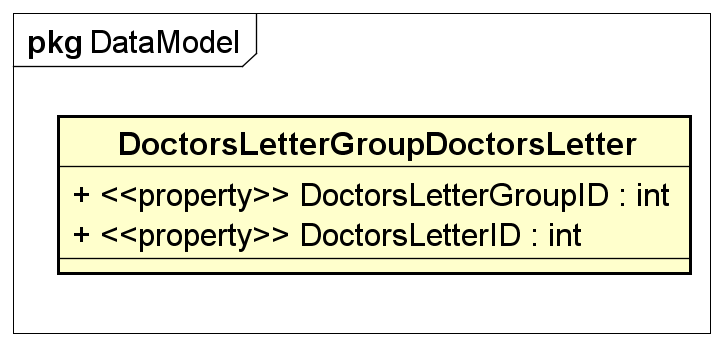
\includegraphics[width=0.75\textheight]{graphics/Klassendiagramme/Model/DoctorsLetterGroupDoctorsLetter.png}
\caption{DoctorsLetterGroupDoctorsLetter Klasse}
\end{figure}
\textbf{Art der Änderung:} Neue Klasse

\textbf{Beschreibung:} Um Many-To-Many Relationen darstellen zu können, benötigt das SQLite-net-extensions Framework eine separate Klasse für die Relation. Da Arztbriefe und Gruppen in einer solchen Relation stehen wird diese Klasse benötigt.

\textbf{Paket:} Model.DataModel

\subsubsection{IFileHelper}
\begin{figure}[H]
\centering
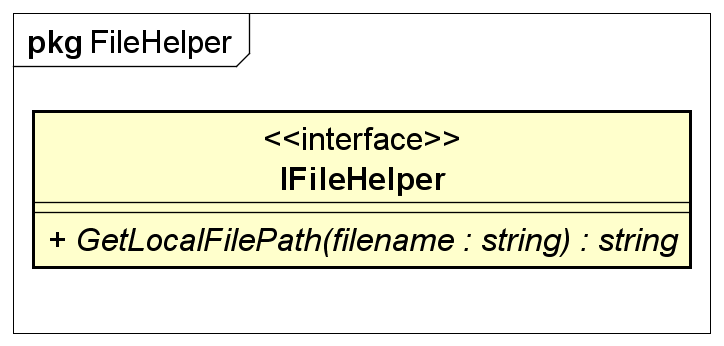
\includegraphics[width=0.75\textheight]{graphics/Klassendiagramme/Model/IFileHelper.png}
\caption{IFileHelper Schnittstelle}
\end{figure}
\textbf{Art der Änderung:} Neue Methode

\textbf{Beschreibung:} Methode zum Löschen von Dateien hinzugefügt.

\textbf{Paket:} Model.FileHelper

\section{Nicht umgesetzte Kriterien}
\textit{Hinweis: Manche dieser Kriterien (z.B. [PK2030]) wurden nur teilweise umgesetzt. D.h. nur manche Teile unseres Projektes unterstützen diese Kriterien, aber aus Zeitgründen wurde die vollständige Implementierung verschoben. Die halbfertigen Kriterien werden durch ein \dq{}!\dq{} gekennzeichnet.}
\subsubsection{Patientenseitige Datenübertragung}
\begin{tabular}{lll}
{[WK1010]} & \multicolumn{2}{p{12cm}}  {Ein \gls{Arztbrief} kann von der myMD \gls{App} des Patienten auf die \gls{Desktop Anwendung} übertragen werden.} \\
{[WK1020]} & \multicolumn{2}{p{12cm}}  {Der Patient kann mehrere \glspl{Arztbrief} gleichzeitig senden.} \\
{[WK1030]} & \multicolumn{2}{p{12cm}}  {\gls{NFC} steht als weitere Übertragungsmöglichkeit zur Verfügung.} \\
{[WK1040]} & \multicolumn{2}{p{12cm}}  {Der Patient wird vor dem Senden von sensiblen Daten darauf hingewiesen, dass er sensible Daten versendet.} \\
{[WK1050]} & \multicolumn{2}{p{12cm}}  {Ein Profil auf einem Mobilgerät kann auf ein anderes übertragen werden.} \\

\end{tabular}

\subsubsection{Darstellung}
\begin{tabular}{lll}
{![PK2030]} & \multicolumn{2}{p{12cm}}  {Die Darstellung eines Arztbriefes umfasst verordnete \gls{Medikament}e.} \\
{[WK2020]} & \multicolumn{2}{p{12cm}}  {Laborwerte des Patienten werden in einem extra \gls{Tab} chronologisch absteigend sortiert dargestellt.} \\
{[WK2030]} & \multicolumn{2}{p{12cm}}  {Ein \gls{Arztbrief} kann Bilddateien enthalten und die myMD \gls{App} kann diese originalgetreu darstellen und einem \gls{Arztbrief} zuordnen.} \\
{[WK2040]} & \multicolumn{2}{p{12cm}}  {Es gibt die Möglichkeit, \glspl{Arztbrief} nach eigenen Kriterien (Arzt, Krankheit o.ä.) zu gruppieren.} \\
\end{tabular}

\subsubsection{Einstellungen}
\begin{tabular}{lll}
{![WK3010]} & \multicolumn{2}{p{12cm}}  {Auf einer myMD \gls{App} können mehrere \gls{Nutzer} verwaltet werden.} \\
{![WK3030]} & \multicolumn{2}{p{12cm}}  {Der \gls{Nutzer} kann einzelne \glspl{Arztbrief} oder ganze Gruppen als sensibel markieren.} \\
{[WK3040]} & \multicolumn{2}{p{12cm}}  {Die myMD \gls{App} kann den \gls{Nutzer} an regelmäßige Arzttermine (z.B. Zahnarzt, Augenarzt) erinnern.} \\

\end{tabular}

\subsubsection{\gls{Desktop Anwendung}}
\begin{tabular}{lll}
{![WK4010]} & \multicolumn{2}{p{12cm}}  {Die \gls{Versichertennummer}, die in einem \gls{Arztbrief} auf dem Computer des Arztes eingetragen ist, wird vor dem Senden mit der in der myMD App des Patienten hinterlegten \gls{Versichertennummer} abgeglichen und nur bei Übereinstimmung wird der \gls{Arztbrief} gesendet.} \\
\end{tabular}

\subsubsection{Kompatibilität}
\begin{tabular}{lll}
{[WK5020]} & \multicolumn{2}{p{12cm}}  {Die \gls{Desktop Anwendung} wird zusätzlich von macOS 10.12 (und höher) unterstützt.} \\
{[WK5030]} & \multicolumn{2}{p{12cm}}  {Die myMD \gls{App} kann \gls{Arztbrief}e im .pdf Dateiformat anzeigen.} \\
{[WK5040]} & \multicolumn{2}{p{12cm}}  {Die myMD \gls{App} kann \gls{Arztbrief}e im .csv Dateiformat anzeigen.} \\

\end{tabular}
\section{Klassendiagramm (Implementierungsphase)}

\chapter{Ergebnisse der Phase}
\begin{figure}
\section{Ablauf}
\begin{minipage}[c]{\textwidth}
\centering
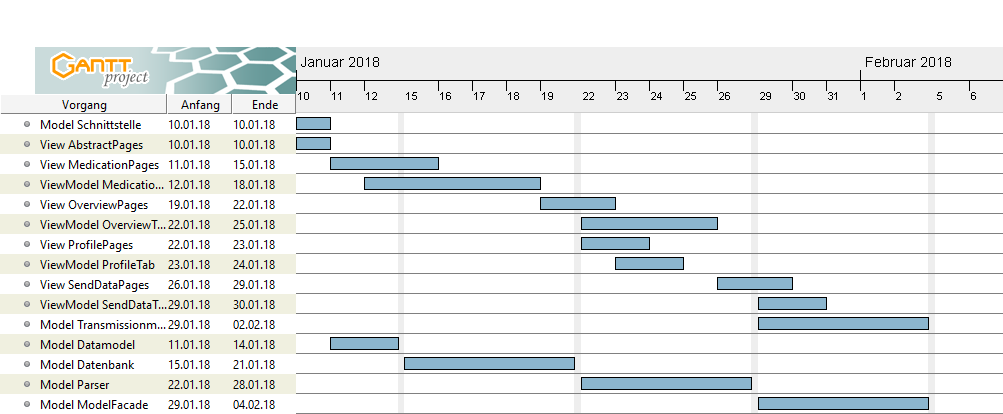
\includegraphics[width=0.95\textheight, angle=90]{Gantt/GanttDiagrammImplementierung}
\caption{Gantt Diagramm der Implementierungsphase}
\end{minipage}
\end{figure}
\section{Zukunftspläne}



\glsaddall
\printnoidxglossaries

% Abbildungsverzeichnis
\listoffigures
 
\end{document}
